\documentclass[5pt]{article}
\usepackage[letterpaper, margin=1in]{geometry}
\usepackage{graphicx}
\usepackage{booktabs}

\begin{document}

\title{Assignment 3}
\author{Mukul Sati [msati3@gatech.edu]}
\maketitle

\section{KNN}
\subsection{Methodology and notation}

I randomly select 20\% of data as test (TtD) and considered the rest as
training data (TD). I select subsets of p\% ($p \in P =\{20, 50, 80, 100\})$
from TD and generate 5 training sets for each of these subsets. The set of
training sets is $TSS = \{TS_1, TS_2, TS_3, TS_4, TS_5\}$. It is these $TS_i$'s
that I do n-fold cross validation on ($n \in N =\{2, 5, 10, |TS_i|\}$). Note
that $|TS_i|$ stands for the cardinality of $TS_i$ and that $|TS_i|$-fold cross
validation corresponds to leave one out cross validation.

Notationally, I carry out several cross validation runs. Each run uses a value
of k ($k \in K$) for the KNN (the set K used is mentioned for each dataset in
the following sections) and carries out n-fold cross validation on a particular
TS generated using a particular percent subset of the TD\@.
$R[p_a,t_b,n_c,k_d]$ refers to the run using the $a^{th}$ indexed element of
$P$, the $b^{th}$ indexed element of $TSS$, the $c^{th}$ indexed element of $N$
and the and the $d^{th}$ indexed element of $K$. For conciseness, in the
remainder of the writeup, I often used the term ``cross validation batch'' to
refer to sets of cross validation runs as determined by conditions on elements
of $P, T, N, K$. For example, the $n$-fold cross validation batch is the set $B
= \{R[p_a,t_b,n_c,k_d] \mid n_c=n, p_a \in P, t_b \in T, k_d \in K\}$. Cross
validation batches are also often expressed by abusing Python's splicing
notation for indexing. Thus, $B = R[:,:,n_c==n,:]$ or even more shorthand, $B =
R[:,:,n,:]$.\\

\noindent \emph{Metric Learning:} I use the metric-learn module
(https://github.com/all-umass/metric-learn) as mentioned by a TA on piazza. I
use the LMNN algorithm to learn a Mahalanobis distance metric.\\

\noindent \emph{Stability:} Each run in the cross validation batch $R[p,:,n,k]$
has an average cross validation error. This is different for each cross
validation run, even with the same $p$ due to differing $TS_i$. Looking at the
average cross validation error for each run as samples of a random variable,
the stability (here tacitly assumed as the inverse of the variance) of the
cross validation error gives some insight on the homogeneity of the dataset and
I comment on this stability for each of the datasets. Intuitively, one would
also expect the variance to decrease with increasing values of $p$, and thus,
the stability to increase with increasing subset sizes used for cross
validation runs. I see if this holds.\\

\noindent \emph{Selecting k:}
The training errors of each batch for a fixed k ($R[:,:,:,k]$) cannot simply be
computed by averaging the training error of each run in the batch, as the runs
are heterogeneous (are obtained from different values of $p$ and $n$). Instead,
I use the box-and-whisker's plot as suggested by a TA to eyeball a good k for
the data-set.\\

\noindent \emph{Testing:}
Now, I train my KNN model using the ``optimal'' value of k using the
entire TD, learning the suitable distance metric and use the trained model for
computing the error on TtD. I compare the this with the cross validated errors,
determining which cross validation split (value of $n \in N$) had given an error
that is most correlated with the error on the test data. The most correlated
$n$ also gives some subtle insight into the distribution of data for the
dataset. Note that for Wine, I use the 20\% split of the data (TtD) for
testing, but for MNIST and office datasets, I use the separate testing data. In
these two cases, I don't split the training data into test and train as the
separate testing data implies no need for hold out testing from the training
set itself (thus TD = all of training data, TtD = $\{\}$ for MNIST and office
datasets).

\subsection{Wine dataset}
\subsubsection{Stability of Cross Validation scores within a TS}
The cross validation scores for the same sized TS ($R[a,:,c,d]$) are similar to
each other, as expected. There is very little variation here, with a maximum
variation in score of 0.017. For the same sized TS, cross validation results
are stable.

\subsubsection{CV scores variation with TS size}
The scores are smaller for smaller sized TD (and thus TS), and greater for
larger sized TD's, as is expected due to larger size of training data being
available for larger TD's. As stated for the same sized TD's but using
different values of $n$ and $k$ are observed to be close, suggesting that the
size of the TS is the most important factor in determining the score. The box
plots described for the selection of best K can be used to see the variation of
CV scores with TS size as well. With increasing TS size, the CV scores become
less varying.

\subsubsection{Best K and associated CV error}
The best k is eyeballed using the box and whisker's plot. Fig
\ref{fig:boxplotsWine} has a couple of them for particular values of k. I have
decided on using k=3 as the best choice. This choice leads to higher scores and
relatively lower variances, but there is not much that can be stated
categorically about my choice as some datapoints as missing (see Discussion).


\begin{figure}[h]
  \center{}
  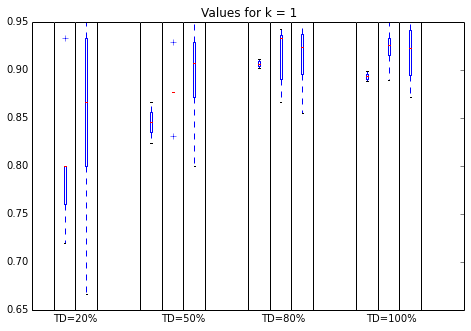
\includegraphics[width=0.4\textwidth]{images/wineBoxK1.png}
  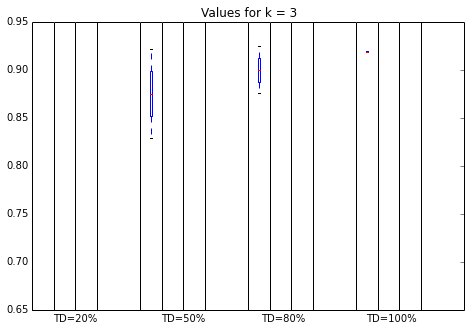
\includegraphics[width=0.4\textwidth]{images/wineBoxK2.png}
  \caption{The box and whisker plots corresponding to k=1(left) and k=3(right)
    for Wine dataset. Note that some data vectors are missing and the reason
    for this is explained in the discussion.}
\label{fig:boxplotsWine} 
\end{figure}

\subsubsection{Testing vs CV}
Using 3 as the KNN k, I get an accuracy of $91.1\%$ on the testing data. This
is most closely correlated with the 5 fold cross validation.

\subsection{MNIST dataset}
For MNIST, I used PCA to reduce dimensionality, retaining enough principal
component vectors that explain 90\% of the variance in the data. I feel this
gives me a good balance between a performant algorithm and execution time.

\subsection{Discussion}
For small dataset such as wine, especially when using a smaller subsampled
dataset, k-fold cross validation is expected to be extremely noisy, more so for
smaller k. In some extreme cases, it may be possible that a k-fold training set
does not contain any data for one class, and thus, no testing data would be
classified to that class. Alternatively, there could be lesser samples in
training for a class than the value of `k' and, in this case, the LMNN
algorithm of metric-learn errors out --- in this case, I've capped the range
of k's tried to the minimum number of training data-points for any class.

\section{HMM}
\subsection{Methodology}
\emph{Modeling:} The training data can be used to constuct the HMM model for
the robot's walks.  Each square in the 4 $\times$ 4 world corresponds to a HMM
state. It is known that the transition probabilities for the non Von-Neumann
neighborhood states (if the states are arranged in a 4 $\times$ 4 matrix) is
zero. The transition probabilities from a particular state to its Von-Neumann
neighbors and to the state itself (to account for black cells) can be computed
using the training data by frequency counting of the transitions. Notationally:

\begin{equation}
a_{ij} = \frac{\#i \rightarrow j}{\sum_{k=1}^{n}\#i \rightarrow k}
\end{equation}

Here we use some of the notation from~\cite{rabiner1989tutorial} for the matrix
of state transition probabilities, and $\#i \rightarrow j$ stands for the
number of times a transition from state i is made to state j. Thus, the
transition matrix can be determined --- this is known to be sparse and thus,
the computations can be made computationally efficient.

The observation at each state if one of the colors $\{r, g, b, y\}$. The
observation can be modeled as a discrete random variable and the probability
distribution for each state can be found by a similar frequency counting of the
training data as for the transition matrix computation. The initial state
probabilities is computable similarly, thus completing the description of the
HMM for the experiment. \\

\noindent \emph{Most probable states:}

\subsection{Results}

\noindent \emph{Learned Model:} The start state probabilities, the state
transition probabilities and the observation symbol probabilities at each state
was learned using training data as described above. I only visualize the
observation probabilities that are learned as described below.

\noindent \emph{Observation Probabilities:} The observation probabilities may
be visualized in a grid for the training data. This is shown in Fig.
\ref{fig:observationP}. Note that the observation propabilities match closely
the sample output of the world as given in the assignment statement.

\begin{figure}[h]
  \center{}
  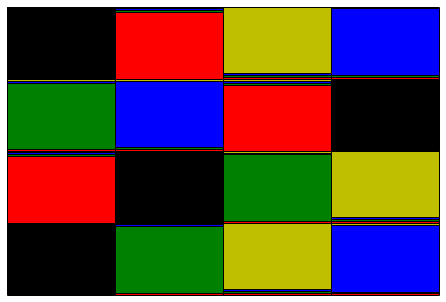
\includegraphics[width=0.5\textwidth]{images/observationP.png}
\caption{The observation probabilities visualized in a grid for the training
data}
\label{fig:observationP}
\end{figure}

\noindent \emph{Hidden State Inference:} Using just the color observation of
each step of a testing random walk, the learned model is used to infer the
state transitions that best explain the walk. This problem displays optimal
substructure, and the Viterbi algorithm provides a dynamic programming solution
for it.

\medskip
\bibliographystyle{unsrt}
\bibliography{references}

\end{document}
